\documentclass[sigconf,nonacm]{acmart}
\usepackage{xeCJK}
\setCJKmainfont{Noto Serif CJK SC}
\setCJKsansfont{Noto Sans CJK SC}
\usepackage{booktabs}
\usepackage{graphicx}
\usepackage{xcolor}
\settopmatter{printacmref=false}
\renewcommand\footnotetextcopyrightpermission[1]{}
\pagestyle{plain}
\newcommand{\todo}[1]{{\color{brown}\textsf{[TODO: #1]}}}
\newcommand{\claim}[1]{} % Source index: claims.md; never prints in the paper.
\emergencystretch=2em
% Generated by scripts/prepare_data.py from existing CSV.
\newcommand{\BSlowMin}{14.8}
\newcommand{\BSlowMax}{17.6}
\newcommand{\APenaltyMin}{9.7}
\newcommand{\APenaltyMax}{10.0}
\newcommand{\BaseWalkFour}{0}
\newcommand{\BaseWalkEight}{65}
\newcommand{\WideWalkFour}{322}
\newcommand{\WideWalkEight}{326}
\newcommand{\FineWalkFour}{0}
\newcommand{\FineWalkEight}{8}
\newcommand{\WideTimeFour}{234869}
\newcommand{\WideTimeEight}{235189}
\newcommand{\BaseTimeFour}{199740}
\newcommand{\BaseTimeEight}{204875}
\newcommand{\FineTimeFour}{198241}
\newcommand{\FineTimeEight}{198930}
\newcommand{\WideA}{194749}
\newcommand{\FineAFour}{213675}
\newcommand{\FineAEight}{214261}
\newcommand{\AWalks}{128}
\newcommand{\UnmapWalkFour}{193}
\newcommand{\UnmapTimeFour}{218700}
\newcommand{\UnmapWalkEight}{197}
\newcommand{\UnmapTimeEight}{219020}
\newcommand{\BatchSixteenInv}{136}
\newcommand{\BatchSixteenFence}{272}
\newcommand{\BatchSixteenFour}{10.3}
\newcommand{\BatchSixteenEight}{7.7}
\newcommand{\BatchSixtyFourInv}{130}
\newcommand{\BatchSixtyFourFence}{260}
\newcommand{\BatchSixtyFourFour}{9.7}
\newcommand{\BatchSixtyFourEight}{7.1}
\newcommand{\MainCases}{24}
\newcommand{\ControlCases}{4}
\newcommand{\MLStrictBFour}{204205}
\newcommand{\MLStrictAFour}{164845}
\newcommand{\MLStrictSlowFour}{2.235}
\newcommand{\MLDeadFour}{46.819}
\newcommand{\MLStrictBEight}{209940}
\newcommand{\MLStrictAEight}{144795}
\newcommand{\MLStrictSlowEight}{2.472}
\newcommand{\MLDeadEight}{36.028}
\newcommand{\MLFQPeak}{128}
\newcommand{\MLFQCapacity}{255}
\newcommand{\MLFQDrain}{501475}
\newcommand{\MLFQTimeout}{500000}
\newcommand{\DiagADelta}{19512}
\newcommand{\DiagFlushDelta}{37854}
\newcommand{\DiagFetchDelta}{38503}
\newcommand{\DiagPTWDelta}{-8503}
\newcommand{\DiagOtherDelta}{-9517}
\newcommand{\DiagHostDelta}{-322}

\title{Cross-Device Translation Interference in a RISC-V IOMMU:\\A Cycle-Level Characterization}
\author{Author information pending}
\affiliation{\institution{\todo{需要作者决定: authors, affiliations, contact email}}\country{}}
\renewcommand{\shortauthors}{Draft authors}

\begin{document}
\begin{abstract}
A shared input/output memory management unit (IOMMU) can expose one device's address translations to another device's invalidations and replacement activity.\claim{C001}
We characterize these effects using existing cycle-level simulations of direct memory access (DMA) engines and a RISC-V IOMMU, with a memory command queue and passive translation tracing.\claim{C002}
In the tested synthetic copies, broad invalidation increases a persistently mapped neighbor's completion time by \BSlowMin\%--\BSlowMax\%, including across distinct first-stage address spaces.\claim{C003}
Context-scoped invalidation across domains, or context-and-address-scoped invalidation within a domain, eliminates invalidation-attributed misses, while increasing the initiator's completion time by \APenaltyMin\%--\APenaltyMax\% relative to broad invalidation.\claim{C004}
Batching unmaps provides partial relief because map-side invalidations remain.\claim{C005}
A separate ablation shows that our platform's way-masked tree-PLRU extension underuses its nominal partition capacity; changing its replacement policy reduces completion time by 12.44\%--22.37\% in the affected case.\claim{C006}
This masked-tree problem does not apply to the upstream unpartitioned implementation.\claim{C007}
Mainline Linux already supports address-scoped and deferred invalidation; this study quantifies policy choices rather than identifying a mainline defect.\claim{C008}
In a separate mainline-derived model, strict unmap increases neighbor time by 2.24\%--2.47\%; deferred flushing and ideal dead-entry removal match the no-invalidation baseline within the short working window.\claim{N001}
The results use behavioral memory timing, with neither CPU nor Linux execution, and do not establish hardware or application performance.\claim{C009}
\end{abstract}
\keywords{RISC-V, IOMMU, DMA, translation cache, invalidation, RTL simulation}
\maketitle

\section{Introduction}
An input/output memory management unit (IOMMU) translates device-visible input/output virtual addresses (IOVAs), using page tables and cached translations~\cite{riscv_iommu_spec2026}.\claim{C010}
When direct memory access (DMA) engines share this structure, a neighbor can lose translations through replacement or through an invalidation whose scope includes its address space.\claim{C011}
These mechanisms call for different remedies: reserving cache entries addresses replacement eligibility, whereas invalidation scope determines which resident entries software removes.\claim{C012}
Prior work studies IOMMU translation costs, sequential ring-buffer translation, translation prefetching, and translation-aware memory scheduling~\cite{iotlb_bottleneck2010,riommu2015,socdma2018,mask2018}.\claim{C013}
Our question is concrete: in one open RISC-V implementation, which shared-translation paths affect a neighbor, by how much under a fixed workload, and with what completion cost to the initiator?

We use the DMA and IOMMU components of a CVA6-based platform, with real register accesses and command-queue fetches in register-transfer-level (RTL) simulation.\claim{C014}
The main experiment preserves the upstream translation-cache and command-handler logic while holding documented platform adaptations and functional fixes constant.\claim{C015}
It compares a no-invalidation baseline against broad, PSCID-scoped, address-scoped, and delayed-unmap invalidation.\claim{C016}
Passive observation records actual resident-entry removal and the first subsequent miss, allowing a distinction between invalidation-attributed misses and other misses.\claim{C017}

The principal result is conditional: broad invalidation dominates the neighbor's translation interference in this workload, even with separate host domains.\claim{C018}
Narrowing its scope protects the neighbor but increases the initiating device's complete time in these runs.\claim{C019}
We also report a separate partition-extension ablation as a design caution: a way mask on a tree replacement policy can provide less effective residency than its nominal quota suggests.\claim{C020}
These are characterization results; they establish neither a new replacement algorithm nor performance across IOMMU implementations.

The Linux distinction is central to the claim. At the audited mainline revision, ordinary invalidation already uses PSCID and address scope, with domain-scoped fallback and deferred-flush support; broad host invalidation is the behavior of the audited development branch and local derivative.\claim{C021}
The paper quantifies the consequences of those choices rather than presenting broad invalidation as a defect in current mainline Linux.

\section{Background}
\subsection{Translation and invalidation scope}
The RISC-V IOMMU specification defines device contexts, first-stage process soft-context identifiers (PSCIDs), guest soft-context identifiers (GSCIDs), and a memory-resident command queue (CQ)~\cite{riscv_iommu_spec2026}.\claim{C022}
We call the implementation's translation cache the I/O translation lookaside buffer (IOTLB). A miss can invoke its page-table walker (PTW).\claim{C023}
For \texttt{IOTINVAL.VMA}, AV, PSCV, and GV indicate valid address, PSCID, and guest-context selectors, respectively.\claim{C024}
With second-stage translation disabled, \texttt{AV/PSCV/GV=0/0/0} invalidates all host address spaces; GV=0 ignores GSCID.\claim{C025}
Consequently, assigning different host PSCIDs does not isolate broad invalidation, and assigning different GSCIDs is not a host-domain solution.\claim{C026}
PSCID-scoped \texttt{0/1/0} selects one host address space, while \texttt{1/1/0} additionally selects the IOVA; both exclude global page-table entries.\claim{C027}
Our mappings have the global bit clear and second-stage translation set to Bare.\claim{C028}

\subsection{Linux DMA mappings and completion}
The audited local DMA-IOMMU path maps a region through \texttt{iommu\_map}, invokes a map synchronization callback, and synchronizes strict unmap; successful maps therefore also generate invalidations.\claim{C029}
For its ordinary host path with Address Translation Services (ATS) disabled, each map or unmap region issues one invalidation and two IOFENCE commands.\claim{C030}
The audited mainline source sets PSCID and supports address invalidation. Its range-command path has priority when supported; otherwise the single-address path falls back to domain scope when its computed count is zero or exceeds 512, with further non-leaf capability conditions~\cite{linux_riscv_mainline2026}.\claim{C031}
This is not a threshold for invalidating all devices. Mainline also supports deferred flushing through its generic page-table domain integration, subject to strict-mode configuration and allocation success.\claim{C032}
These statements describe the frozen source revision, not a kernel executed in our simulation.\claim{C033}
For an ordinary empty-slot 4\,KiB map, that mainline path does not flush; strict unmap uses an address-and-PSCID invalidation followed by one PR=PW=1 IOFENCE.\claim{N002}
RISC-V's policy choice defaults to strict, but this does not establish that DMA-IOMMU is compiled in: if it is absent, the core defaults to an identity domain.\claim{N003}

IOFENCE completion must be interpreted against the implementation. The original handler advances CQ head when it fetches a command, before decoding it, and does not implement the PR/PW read/write-drain requests.\claim{C034}
The driver model uses an invalidation followed by two AV=0 fences, polling the head after each submission; fetching the second fence in this serial, ATS-disabled handler establishes completion of the preceding invalidation/fence sequence.\claim{C035}
Unmap follows confirmed DMA completion, with PR=PW=0; this is a limited completion protocol, not a full IOFENCE conformance result.\claim{C036}

\section{Methodology}
\subsection{Platform and experimental boundaries}
The parent platform integrates CVA6, four iDMA engines, and a RISC-V IOMMU; the reported invalidation test instantiates two real iDMA engines and the full IOMMU command/translation path.\claim{C037}
Figure~\ref{fig:platform} separates this exercised path from the parent platform's CPU/Linux context. The CPU and Linux do not run: a test driver schedules software operations, updates page tables in model memory, and performs real AXI register accesses.\claim{C038}
The baseline uses an unpartitioned 16-entry tree-PLRU IOTLB without hit bypass.\claim{C039}
Its frozen IOMMU revision includes fixes for write routing/progress, page-table leaf handling, counters, and AXI boundary handling; the common write-priority fix can affect service order.\claim{C040}
The CQ handler and IOTLB logic are byte-identical to the selected upstream implementation. This is an adapted and corrected baseline, not a claim that an unmodified complete upstream SoC was evaluated.\claim{C041}

\begin{figure}[t]
  \centering
  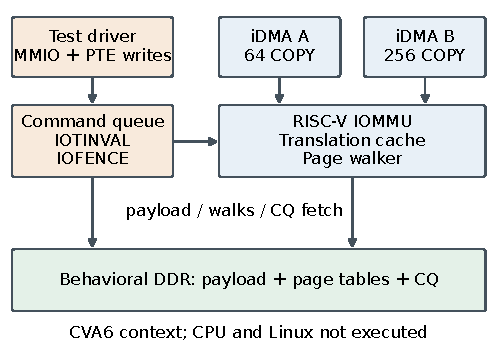
\includegraphics[width=\columnwidth]{figures/platform.pdf}
  \Description{Two DMA engines and a software test driver share the IOMMU and behavioral memory. CPU and Linux are platform context only.}
  \caption{Exercised request path. Software operations come from the test driver; DMA, IOMMU translation, and CQ command fetches use RTL. The workload counts are read from the existing result CSV. The CPU/Linux context is not executed.\claim{F001}}
  \label{fig:platform}
\end{figure}

The behavioral DDR model has one FIFO read-return queue without ID-based reordering; the head waits 16 cycles, then returns an 8-byte beat per cycle.\claim{C042}
For an empty queue with the receiver ready, address acceptance to the first read response is 17 cycles, not 16.\claim{C043}
All invalidation modes use this same deterministic model. Cycles below are simulation clock steps, without conversion to seconds or FPGA timing.\claim{C044}

\subsection{Workload and comparisons}
Initiator A performs 64 aligned 4\,KiB COPY operations; neighbor B performs 256, retaining a fixed source and either three or seven destination pages, for four- or eight-page footprints.\claim{C045}
Each A copy maps and unmaps its source and destination regions. A uses fresh descending IOVAs and does not recycle physical pages during the test.\claim{C046}
B first executes 64 warm-up copies, followed by residency checks and destination coverage checks with zero additional walks; this warm-up is outside the common measurement start.\claim{C047}
The main window retains A's cold translations and all measured command/DMA activity.\claim{C048}
Same-domain cases share the first-stage root and PSCID; different-domain cases use distinct roots and PSCIDs.\claim{C049}

M0 persistently maps all A pages before the window and issues no invalidations inside it. It retains A's streaming replacement pressure, so it is a no-invalidation comparison rather than a reproduction of map/unmap software costs.\claim{C050}
M1 uses broad invalidation on every map and unmap. M2 scopes each operation to A's PSCID, and M3 scopes it to both A's PSCID and page address.\claim{C051}
M4 retains broad map-side invalidation but batches unmaps every $N=16$ or $64$ unmapped page regions, draining the remainder at the end and withholding reuse until synchronization.\claim{C052}
Those batch sizes model bounded delayed unmap, not Linux's actual default timer/ring policy, and do not imply that the local development driver supports deferred flushing.\claim{C053}
The original matrix contains \MainCases{} configurations and \ControlCases{} controls that suppress map-side flushing; each recorded configuration was executed once.\claim{C054}

The separate mainline-derived study assumes enabled DMA-IOMMU, translated domains, one CPU's flush queue, and pre-existing page-table levels with leaf-only unmaps.\claim{N004}
Because the original handler omits PR/PW, its test-only overlay holds fence completion until a snapshot of completion-interface accepted AR/AW requests reaches modeled DDR RLAST/write-response completion, used as a conservative global ordering point.\claim{N005}
That completion model is disclosed rather than treated as upstream RTL support or universal hardware timing.\claim{N006}
The snapshot can omit an already translated request waiting before that interface accepts it; no such omission is established for the recorded runs, but the overlay is not a complete PR/PW safety implementation.\claim{N024}

\subsection{Attribution and time accounting}
At each real CQ invalidation, the observer saves resident keys, computes the selected scope, and checks after the edge that the corresponding valid bits cleared.\claim{C055}
The first subsequent miss to such a key is invalidation-attributed; previously unseen keys are cold, and remaining misses without an invalidation mark are classified as replacement misses.\claim{C056}
This is an operational classification of misses, not an additive causal decomposition of completion time. Lookup episodes and accepted walk starts are counted separately.\claim{C057}
Raw event and per-copy records check complete data coverage, read/write beats, write responses, and hardware completion; a final DONE flag alone is insufficient.\claim{C058}

We report $T_A$ from the common start through A's last unmap/fence completion, and $T_B$ through B's last hardware COPYDONE.\claim{C059}
The joint makespan is $\max(T_A,T_B)$; adding the two device times is a different measure.\claim{C060}
The test includes MMIO polling, CQ fetches, DMA, and model-memory cycles, but excludes CPU execution time for page-table updates.\claim{C061}
Frozen source manifests, per-run identities, summaries, and compressed raw traces are retained with the existing results.\claim{C062}

\section{Results}
\subsection{Broad invalidation reaches the neighbor}
Figure~\ref{fig:neighbor} normalizes B's complete time to M0 with the same footprint and domain relation.\claim{F002}
M0 takes \BaseTimeFour{} and \BaseTimeEight{} cycles for the four- and eight-page footprints, with \BaseWalkFour{} and \BaseWalkEight{} walks, respectively.\claim{C063}
M1 increases completion time to \WideTimeFour{} and \WideTimeEight{} cycles, or \BSlowMax\% and \BSlowMin\%.\claim{C064}
Its \WideWalkFour{} and \WideWalkEight{} walks are all invalidation-attributed misses; the M0 walks are not.\claim{C065}
The different-domain and same-domain measurements are identical for broad invalidation, consistent with its all-host scope.\claim{C066}
Domain separation therefore provides no invalidation isolation for M1 in this host first-stage configuration.\claim{C067}

\begin{figure}[t]
  \centering
  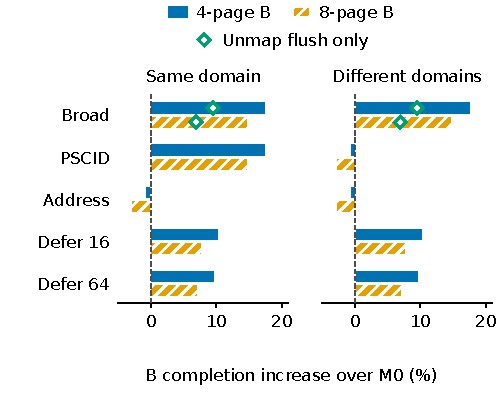
\includegraphics[width=\columnwidth]{figures/invalidation_neighbor.pdf}
  \Description{B slowdown relative to the same-domain and footprint no-invalidation baseline for broad, PSCID, address, and delayed unmap policies.}
  \caption{Neighbor B completion normalized to matching M0. Domain relation and footprint are kept explicit; M2 protects B only across distinct PSCIDs. M4 batches unmaps while retaining map-side broad invalidation.\claim{F003}}
  \label{fig:neighbor}
\end{figure}

M2 leaves the same-domain neighbor as exposed as M1, but across domains it eliminates invalidation-attributed misses; M3 does so for both domain relations.\claim{C068}
The protected cases have \FineWalkFour{} and \FineWalkEight{} total B walks and complete in \FineTimeFour{} and \FineTimeEight{} cycles.\claim{C069}
The eight-page residual walks are classified as replacement, so zero invalidation misses does not mean zero misses overall.\claim{C070}
The lower eight-page walk count than M0 reflects a changed replacement history, not an additional category of negative invalidation misses; the dead-entry control below tests a narrower explanation.\claim{C071}

\subsection{Protecting B changes A's completion cost}
Figure~\ref{fig:initiator} includes A's final synchronization.\claim{F004}
M1 takes \WideA{} cycles for A, whereas the protective M2/M3 cases take \FineAFour{} or \FineAEight{} cycles, increasing $T_A$ by \APenaltyMin\%--\APenaltyMax\%.\claim{C072}
A's walk count stays at \AWalks{}, and the fine-scope and broad per-operation modes issue the same numbers of invalidation and fence commands.\claim{C073}
Thus fewer neighbor misses do not, by themselves, predict a shorter initiator completion time.\claim{C074}
Follow-up diagnosis retains the original PR=PW=0, two-fence protocol: when A runs alone, broad and fine invalidations take the same 62 cycles from submission through first-fence completion in every recorded round.\claim{N007}
With the eight-page neighbor, the protective mode adds \DiagADelta{} A cycles; its flush-busy occupancy rises by \DiagFlushDelta{}, including \DiagFetchDelta{} more cycles in CQ FETCH/REGISTER, while PTW, other-copy, and host/configuration occupancy fall.\claim{N008}
The complete mode difference is therefore a co-run interaction, also conditioned on B's warm prefix, rather than extra invalidation-decode cycles; these occupancy differences are not individually recoverable causal costs.\claim{N009}
In particular, this diagnosis does not measure PR/PW drain, which was disabled in these runs.\claim{N010}

\begin{figure}[t]
  \centering
  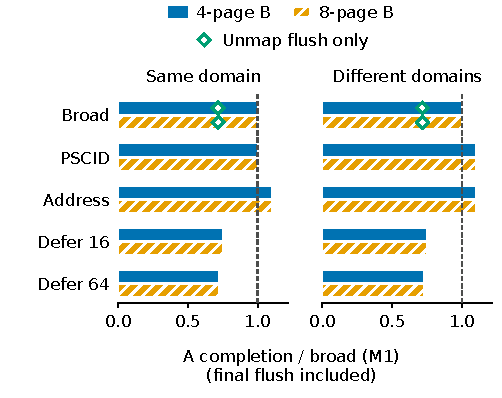
\includegraphics[width=\columnwidth]{figures/invalidation_initiator.pdf}
  \Description{A completion including final synchronization relative to broad invalidation, separately for same and different domains and two B footprints.}
  \caption{Initiator A completion including final unmap/fence, with M1 as the reference. These original policies use PR=PW=0 and two fences per flush; they are distinct from the mainline-derived model.\claim{F005}}
  \label{fig:initiator}
\end{figure}

\subsection{Delayed unmap only partly mitigates broad flushing}
Table~\ref{tab:commands} reports measured command counts, walks, and A time.\claim{T001}
M4 reduces invalidation/fence counts from 256/512 to \BatchSixteenInv{}/\BatchSixteenFence{} at $N=16$, or \BatchSixtyFourInv{}/\BatchSixtyFourFence{} at $N=64$.\claim{C075}
B still exceeds M0 complete time by \BatchSixteenEight\%--\BatchSixteenFour\% and \BatchSixtyFourEight\%--\BatchSixtyFourFour\%, respectively.\claim{C076}
Batching unmap therefore only partly addresses the broad-flush interference in this test.\claim{C077}
In the separate unmap-only-flush controls, B has \UnmapWalkFour{}/\UnmapWalkEight{} walks and \UnmapTimeFour{}/\UnmapTimeEight{} cycles, compared with M1's \WideWalkFour{}/\WideWalkEight{} walks and \WideTimeFour{}/\WideTimeEight{} cycles.\claim{C078}
Omitting map-side flushing materially changes the measurement; these controls isolate a component and do not replace the full map/unmap path.\claim{C079}

\begin{table}[t]
  \centering
  \footnotesize
  \caption{Command and completion accounting from the existing CSV. A time includes final synchronization. M2 here uses distinct domains; same-domain M2 equals M1. M3 values hold for both domain relations.\claim{T002}}
  \label{tab:commands}
  \begin{tabular}{lrrr}
\toprule
Mode & IOTINVAL / fences & B walks & $T_A$ (cycles) \\
 & & (4 / 8 pages) & (4 / 8 pages) \\
\midrule
M0 & 0 / 0 & 0 / 65 & 81,739 / 86,639 \\
M1 & 256 / 512 & 322 / 326 & 194,749 / 194,749 \\
M2, different & 256 / 512 & 0 / 8 & 213,675 / 214,261 \\
M3 & 256 / 512 & 0 / 8 & 213,675 / 214,261 \\
M4, $N=16$ & 136 / 272 & 210 / 214 & 145,718 / 145,718 \\
M4, $N=64$ & 130 / 260 & 198 / 202 & 140,756 / 140,756 \\
\bottomrule
\end{tabular}

\end{table}

\subsection{Mainline-derived policies and dead translations}
The mainline-derived strict policy gives B \MLStrictBFour{} and \MLStrictBEight{} cycles, \MLStrictSlowFour\% and \MLStrictSlowEight\% above M0; same- and different-domain values are identical.\claim{N011}
A completes in \MLStrictAFour{} and \MLStrictAEight{} cycles, including its final unmap synchronization.\claim{N012}
Figure~\ref{fig:mainline} distinguishes these results from the development-policy matrix: map flushing, fence count, and PR/PW semantics all differ, so the comparison is not an isolated change of scope bits.\claim{N013}

ML-FQ uses a deferred flush queue (FQ) for unmap synchronization; ORACLE adds immediate, wait-free invalidation of dead A entries to otherwise identical FQ behavior.\claim{N014}
Both match M0's B times, \BaseTimeFour{} and \BaseTimeEight{}, so ORACLE improves B completion by 0\% over FQ in all four domain/footprint cases.\claim{N015}
FQ's mean dead occupancy is nevertheless \MLDeadFour\%/\MLDeadEight\% of all sixteen slots.\claim{N016}
The tested PLRU victim selection does not consult valid bits, and clearing never-revisited A entries changes neither subsequent active hits nor replacement choices; the paired service traces are cycle-identical.\claim{N017}
Thus this particular dead-entry population is not evidence of recoverable performance loss, and the result does not motivate a dead-entry hint mechanism.\claim{N018}

The deferred queue reaches only \MLFQPeak{} entries against \MLFQCapacity{} usable entries, and both devices finish before its first 10\,ms timer deadline.\claim{N019}
The timer is modeled as \MLFQTimeout{} cycles under a declared 50\,MHz/HZ=1000 equivalence; subsequent flushing completes at cycle \MLFQDrain{}, reported separately from A's earlier API completion.\claim{N020}
This short workload does not measure interference from periodic FQ flushing or a full queue.\claim{N021}
The reverse effect of a global PR/PW fence making the unmapping device wait for a neighbor remains unmeasured; the legacy diagnosis does not establish it.\claim{N026}

\begin{figure}[t]
  \centering
  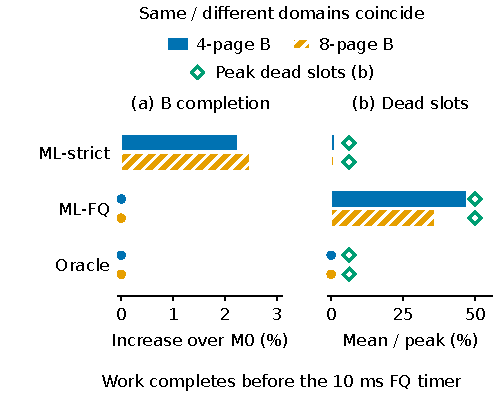
\includegraphics[width=\columnwidth]{figures/mainline_baseline.pdf}
  \Description{Mainline-derived strict, deferred flush and immediate dead-entry removal compared against the no-invalidation baseline under both B footprints.}
  \caption{Mainline-derived model under explicit DMA-IOMMU assumptions and a test-only PR/PW completion overlay. FQ and ORACLE match M0 during a window that ends before the first timer flush; this is not a steady-state FQ result.\claim{F007}}
  \label{fig:mainline}
\end{figure}

\subsection{A separate trap in partitioned tree-PLRU}
The replacement ablation uses a different fixture: P assigns two entries to the neighbor and fourteen to A; PN additionally enables an early hit bypass. Both retain the fixture's common pre-commit data-structure-first arbitration rule.\claim{C080}
Each device performs 64 copies, and A cycles through $R$ destination pages with a fixed source; complete time includes cold initialization, configuration, refill, completion discovery, and final quiescence.\claim{C081}
These measurements cannot be merged numerically with the unpartitioned invalidation baseline.\claim{C082}

At $R=8$, A's nine-page footprint causes 37 walks and the two devices together cause 39 under the original masked tree (V0).\claim{C083}
Direct victim tracing shows A's hot source staying in way 8, all 30 valid evictions targeting ways 2 and 3, and seven eligible entries remaining unused.\claim{C084}
The extension masks eligible ways without rebalancing the underlying tree; the result demonstrates that a fourteen-entry quota does not guarantee nine-page residency for this trace.\claim{C085}
This is our platform's partition extension: the examined upstream implementation has no such way mask and does not have this particular masked-tree problem.\claim{C086}

V1 approximately rebalances the eligible leaves while preserving the prior touch/fill semantics; V2 uses exact least-recently-used replacement, invalid-entry priority, and most-recently-used insertion.\claim{C087}
At $R=8$, total walks fall from 39 to 25 with V1 and to 11 with V2.\claim{C088}
V2 reduces complete time by 12.44\% for P and 22.37\% for PN; at $R=16$, all policies still perform 67 walks and complete time is unchanged.\claim{C089}
Figure~\ref{fig:plru} retains these non-improving cases; the intervention bundles several replacement choices and does not isolate invalid-first insertion alone.\claim{C090}

\begin{figure}[t]
  \centering
  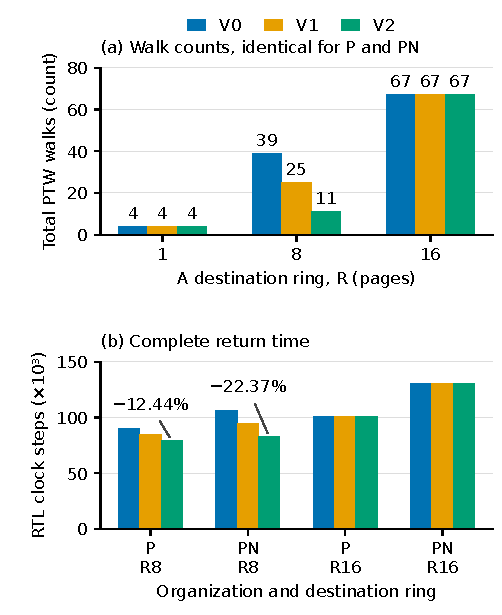
\includegraphics[width=\columnwidth]{figures/plru_ablation.pdf}
  \Description{Three replacement variants reduce R8 walks from39 to25 to11; R16 walks remain67. Complete P and PN times improve only in the R8 cases.}
  \caption{Separate partition-extension ablation. V0 is masked tree-PLRU, V1 approximately rebalances eligible leaves, and V2 changes replacement/insertion semantics. Complete time is the fixture's $T_{\mathrm{return}}$, including final quiet; it differs from the main experiment's device times.\claim{F006}}
  \label{fig:plru}
\end{figure}

\section{Discussion}
\subsection{Implications for drivers and IOMMU design}
The tested hardware already supports scoped invalidation, and audited mainline Linux already uses it.\claim{C091}
For a driver designer, these results support auditing actual scope bits, map callbacks, and fallback paths before treating device domains as performance isolation.\claim{C092}
For an IOMMU designer, they support measuring both devices' complete times alongside miss counts and command traffic.\claim{C093}
The observed A penalty makes a miss-only objective incomplete; distinguishing CQ-fetch interference from PR/PW completion effects remains necessary before generalizing the diagnosis.\claim{C094}
For partition design, eligible-entry counts should be accompanied by observed occupancy and victim distributions, and replacement alternatives should be compared with complete-time accounting.\claim{C095}

\subsection{Limitations}
All reported timing comes from RTL simulation with behavioral DDR, not FPGA or physical-memory timing; CPU and Linux execution are absent, and software behavior is supplied by the test driver.\claim{C096}
The synthetic aligned 4\,KiB COPY workloads do not establish application behavior. In particular, A's fresh descending IOVAs can differ from Linux's range-cache reuse, and the batching sizes do not reproduce its timer-driven flush queue.\claim{C097}
The invalidation matrix records one deterministic execution per configuration, so it provides no statistical uncertainty or sensitivity to different memory systems.\claim{C098}
The PLRU fixture has its own service model and research extensions; it provides a local counterexample to quota-based reasoning, not an upstream bug or a general replacement-policy ranking.\claim{C099}
Only one IOMMU implementation is characterized. The replacement, invalidation, and complete-time conclusions cannot be transferred directly to other IOMMUs.\claim{C100}
The mainline-derived baseline models selected source behavior, not a booted default kernel. Its PR/PW completion overlay does not establish a general physical ordering cost, and the global-fence neighbor-wait hypothesis remains pending.\claim{N022}

\section{Related Work}
Early IOTLB work examines DMA mapping costs and cache-management choices; we cite its workshop version~\cite{iotlb_bottleneck2010}.\claim{C101}
rIOMMU uses sequential ring-buffer access to replace hierarchical translation with a circular flat table; Kurth et al. combine compiler-generated translation prefetching, parallel miss helpers, and DMA burst tracking/retry~\cite{riommu2015,socdma2018}.\claim{C102}
MASK addresses translation and memory scheduling across concurrent GPU applications~\cite{mask2018}.\claim{C103}
Our experiments instead quantify invalidation scope and its per-device completion tradeoff in a specific RISC-V IOMMU, and separately expose a platform-specific partition implementation pitfall.\claim{C104}
The RISC-V IOMMU extended abstract provides implementation context, without supplying a performance comparison here~\cite{zero_day_iommu2023}.\claim{C105}
Intel VT-d already specifies domain- and page-selective IOTLB invalidation with scoped read/write-drain guarantees~\cite{intel_vtd2024}; these are minimum completion guarantees, not proof that implementations never wait for other domains.\claim{N025}
We therefore make no novelty claim for adding scoped drain, and report no Intel hardware performance comparison.
\todo{待核文献: complete verified iDMA and CVA6 bibliographic records before adding their scholarly citations.}

\section{Conclusion}
Broad host invalidation, rather than capacity pressure alone, dominates the neighbor's observed translation interference in the tested workload.\claim{C106}
Scoped invalidation removes invalidation-attributed misses and shifts measured completion cost toward the initiator; unmap batching provides partial relief while map-side flushing remains.\claim{C107}
The separate PLRU ablation shows why partition capacity must be checked against actual replacement behavior.\claim{C108}
The mainline-derived short-run result is smaller than the broad-flush result, and ideal dead-entry removal provides no B speedup; periodic FQ and global-fence effects remain outside the established findings.\claim{N023}

\paragraph{Availability and declarations.}
Frozen sources, logs, and analysis inputs are retained locally with the reported runs.\claim{C109}
\todo{需要作者决定: release URL and artifact packaging; author contributions, funding, conflicts of interest, and ethics declaration.}
This draft and its plots were prepared with AI assistance; the authors must review and take responsibility for the submitted version.\claim{C110}

\bibliographystyle{ACM-Reference-Format}
\bibliography{references}
\end{document}
